\begin{figure}[!t]
  \centering
  \begin{subfigure}{\columnwidth}
      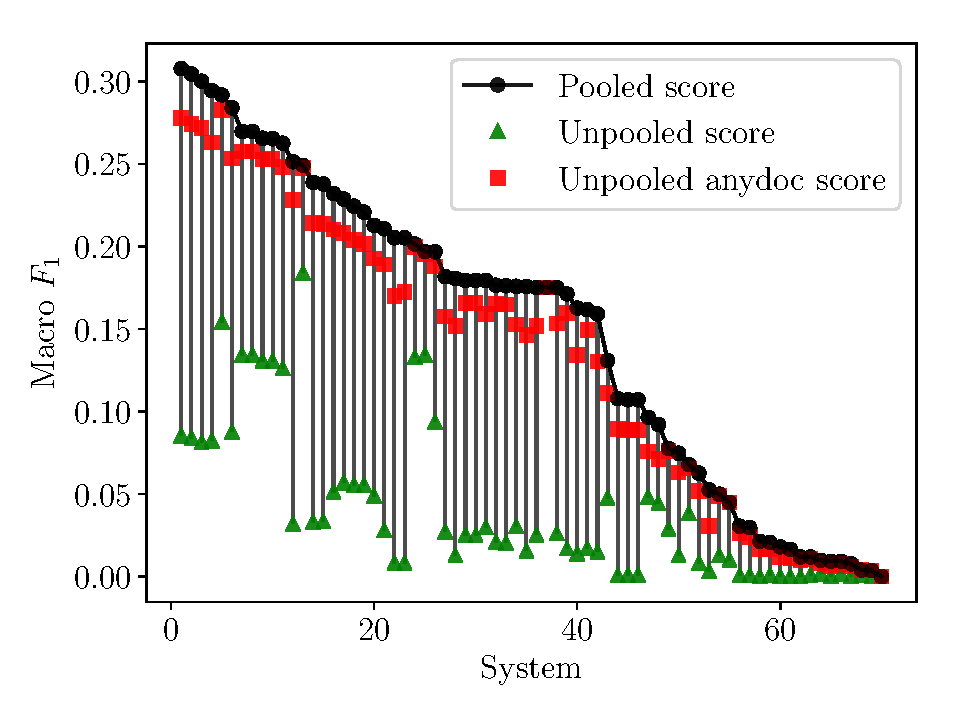
\includegraphics[width=0.8\columnwidth]{figures/pooling_bias_f1/pooling_bias/pooling_bias}
    \centering
    \small{\begin{tabular} {l r r r} \toprule
                    & \multicolumn{3}{c}{Median bias} \\
                    & Precision & Recall & Macro \fone{} \\ \midrule 
   Official         & 17.93\% &  17.00\% & 15.51\% \\ 
   \anydoc{}        & 2.34\% &  1.93\% & 2.05\% \\ \bottomrule
   \end{tabular}}
  \end{subfigure}
  \caption[Pooling bias for \fone{} in TAC-KBP 2015]{\label{fig:pooling-bias} Median pooling bias (difference between pooled and unpooled scores) on the top 40 systems of TAC KBP 2015 evaluation using the official and \anydoc{} scores.
  The bias is much smaller for the lenient \anydoc{} metric, but even so, it is larger than the largest difference between adjacent systems (1.5\% \fone{}) and typical system improvements (around 1\% \fone{}).
%  the assumption that pooling bias is insignificant is false.
  }
\end{figure}

\begin{figure}[!t]
  \centering
  \begin{subfigure}{0.8\columnwidth}
      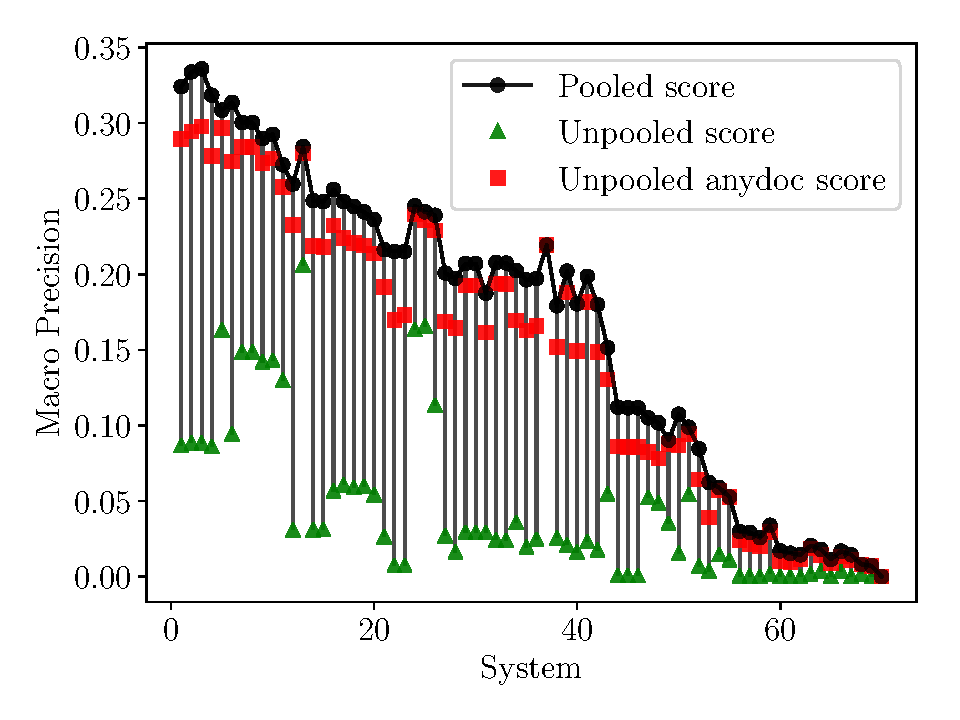
\includegraphics[width=\textwidth]{figures/pooling_bias/pooling_bias_p}
  \end{subfigure}

  \begin{subfigure}{0.8\columnwidth}
      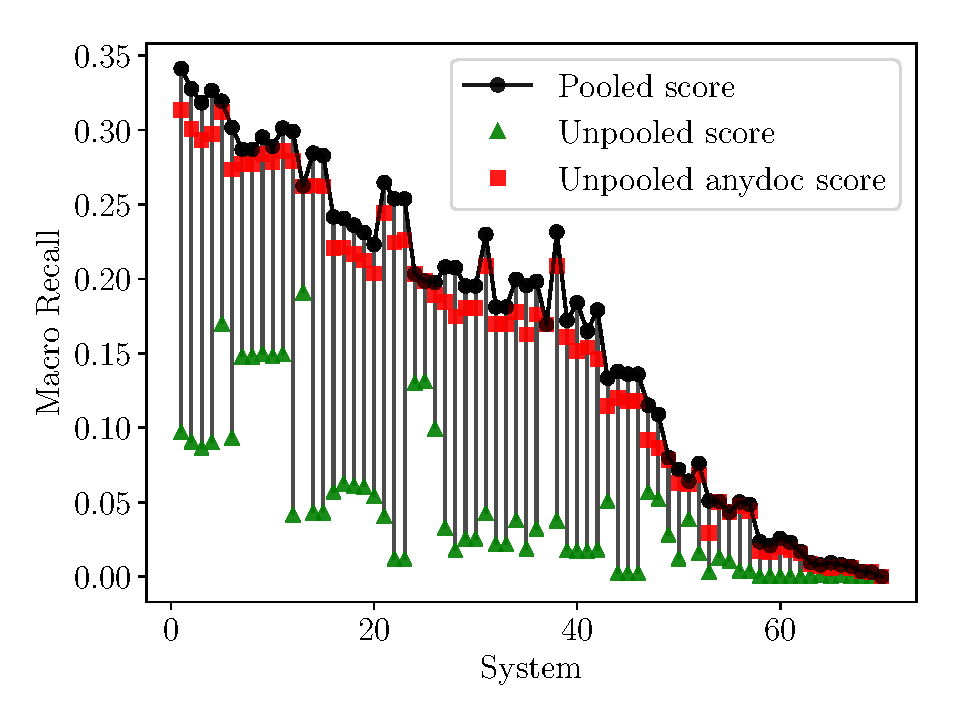
\includegraphics[width=\textwidth]{figures/pooling_bias/pooling_bias_r}
  \end{subfigure}
  \caption[Pooling bias for precision and recall in TAC-KBP 2015]{\label{fig:pooling-bias-p-r} Pooling bias broken down by precision and recall.}
\end{figure}

\section{Measuring pooling bias}
\label{sec:kbpo:analysis}
%(1 pages)

% Primer
The example in \reffig{pooling} makes it apparent that pooling-based evaluation can introduce a systematic bias against unpooled systems.
However, it has been assumed that the bias is insignificant in practice given the large number of systems pooled in the TAC KBP evaluation.
We will now show that the assumption is not valid using data from the TAC KBP 2015 evaluation.\footnote{%
Our results are not qualitatively different on data from previous years of the shared task.}

% Data and methodology
\paragraph{Measuring bias.}
In total, there are 70 system submissions from 18 teams for 317 evaluation entities ($E$) and the evaluation set consists of 11,008 labeled relation instances.\footnote{%
  The evaluation set is actually constructed from compositional queries like, ``what does Carrie Fisher's parents do?'':
  these queries select relation instances that answer the question ``who are Carrie Fisher's parents?'', and then use those answers (e.g.\ ``Debbie Reynolds'') to select relation instances that answer ``what does Debbie Reynolds do?''.
  We only consider instances selected in the first part of this process.
}
The original evaluation dataset gives us a good measure of the true scores for the participating systems.
Similar to \citet{zobel1998reliable}, which studied pooling bias in information retrieval,
we simulate the condition of a team not being part of the pooling process by removing any predictions that are unique to its systems from the evaluation dataset.
The pooling bias is then the difference between the true and unpooled scores.

\paragraph{Results.}
\reffig{pooling-bias} shows the results of measuring pooling bias on the TAC KBP 2015 evaluation on the \fone{} metric using the official and \anydoc{} scores.\footnote{%
  We note that \anydoc{} scores are on average 0.88\%\fone{} larger than the official scores. 
  }\footnote{
  The outlier at rank 36 corresponds to a University of Texas, Austin system that only filtered predictions from other systems and hence has no unique predictions itself.
  }
\reffig{pooling-bias-p-r} further breaks down the results for precision and recall.
We observe that even with lenient \anydoc{} heuristic, the median bias (2.05\% \fone{}) is much larger than largest difference between adjacently ranked systems (1.5\% \fone{}).
This experiment shows that pooling evaluation is significantly and systematically biased against systems that make novel predictions!

